\chapter{تخصیص منابع در شبکه‌های دسترسی رادیویی باز}
\section{مقدمه}
در اینحا هدف ما، فرمول بندی برش RAN برای معماری O-RAN است. این مطالعه، تکنیکی را برای ایجاد خطوط کلی برش شبکه ایزوله در معماری O-RAN برای ارائه QoS خاص برای eMBB، URLLC و mMTC ارائه می‌کند. علاوه بر منابع باند پایه، تعداد VNF ها نیز برای کاهش تأخیر به ویژه برای خدمات URLLC، در نظر گرفته می شود.
در این بخش هدف تخصیص منابع در ساختار شبکه های دسترسی رادیویی باز با استفاده از برش شبکه برای سرویسهای مختلف با کیفیت سرویس متفاوت باتوجه به شکل \ref{fig:c11} می باشد. 
خلاصه‌ی مهم‌ترین نوآوری‌های این بخش بدین صورت است:
\begin{itemize}
	\item 
	در اینجا یک مدل برش شبکه را برای سه سرویس مختلف معرفی شده در \lr{5G}، یعنی eMBB، mMTC و URLLC به تصویر می‌کشد. در معماری O-RAN، مشکل تخصیص منابع رادیویی و فعال سازی VNF بررسی می شود.
	ما بر اساس انواع مختلف خدمات با اولویت ها و QoS مختلف، یک مسئله برای تخصیص منابع باند پایه برای به حداکثر رساندن توان عملیاتی وزنی O-RAN فرموله می کنیم.
	\item 
	ما دراینجا تأخیر پردازش و منابع VNF مورد نیاز برای برش را در مقایسه با سایر مقالات در نظر گرفته‌ایم. بنابراین، ما بر به دست آوردن تعداد بهینه VNF در هر لایه از معماری O-RAN تمرکز می نماییم.
	همچنین سرویسهای مختلف با QoS مختلف شامل تاخیر، توان و نرخ را بررسی نموده‌ایم و با توجه به تعداد VNFهای فعال شده و نرخ هر کابر، تاخیر پردازشی انتها به انتها را بدست می‌اوریم.
	
	با فرض ظرفیت محدود فرانتهال، توان و ظرفیت واقعی هر O-RU را محاسبه می کنیم. بسته به نوع سرویس، تداخل O-RUهای همسایه را مدل کرده و نرخ را تعیین می‌نماییم. در مدل سیستم در نظر گرفته شده، انتقال بسته کوتاه URLLC و mMTC را به حساب می‌آوریم که نمی‌توان با قضیه ظرفیت شانون مدل‌سازی کرد.
\item 	
مسئله‌ی مورد بررسی، یک مسئله‌ی غیرخطی همراه با  ترکیب اعداد صحیح و پیوسته است که برای حل آن از یک الگوریتم دو مرحله‌ای تکراری استفاده می‌نماییم که در مرحله‌ی اول، تعداد VNFهای فعال، تخصیص توان و PRB بدست می‌آید و در مرحله‌ی دوم ارتباط کاربران با o-RU ها بدست می‌آید.
\item 
ما مسئله‌ی اصلی را در مرحله‌ی اول برای یافتن یک کران بالا و پایین برای تعداد VNF های فعال شده مجدداً فرموله و ساده می کنیم و از تابع لاگرانژی و شرایط KKT برای یافتن توان بهینه و تخصیص PRB استفاده می کنیم.
برای مرحله دوم، مسئله‌ی ارتباط O-RU را می توان به یک مسئله‌ی کوله پشتی چندگانه تبدیل کرد و با الگوریتم حریصانه حل کرد.
\item 
در نهایت، بحث در مورد انتخاب نقطه اولیه و منطقه امکان پذیر برای نتایج عددی ارائه شده است. همچنین، ما یک الگوریتم سریع را معرفی می‌کنیم که پیچیدگی کمتری نسبت به روش ما برای تحقق بخشیدن به منطقه امکان‌پذیر برای مسئله‌ی ما دارد. 
\end{itemize} 

\begin{figure}
  \centering
  \captionsetup{justification=centering}
    \includegraphics[scale = 0.4]{./img/finalDraw1.pdf}
    %\includegraphics[width=9.cm,height=6.2cm]{finalDraw1.pdf}
    %\includegraphics[width=\textwidth]{finalDraw.pdf}
  \caption{برش شبکه در سیستم O-RAN}
  \label{fig:c11}
\end{figure}
در ادامه‌ی این فصل، ابتدا مدل سیستم و فرمولاسیون مسئله را بیان می‌نماییم. سپس الگوریتم مورد نظر را ارائه داده و در نهایت     نتایج عددی رو بیان می کنیم.

\section{مدل سیستم و فرمولاسیون مسئله}\label{systemmodel}
در این بخش، سیستم فروسو \LTRfootnote{Downlink} را در معماری O-RAN با استفاده از برش RAN همانطور که در شکل \ref{fig:c11} نشان داده شده است، توصیف می کنیم.
ابتدا مدل سیستم را ارائه می کنیم. سپس، نرخ‌های داده قابل دستیابی، توان O-RU و ظرفیت فرانتهال برای لینک فروسو سیستم O-RAN را به دست می‌آوریم. پس از آن، میانگین تاخیر و توان VNF ها را مورد بحث قرار می دهیم.
در نهایت مسئله‌ی اصلی بیان می شود.
\subsection{مدل سیستم}
فرض کنید، سه نوع سرویس شامل eMBB، URLLC و mMTC وجود دارد که از برنامه های مختلف پشتیبانی می کنند.
بر این اساس، برش‌های $S_1$ برای نوع سرویس اول (eMBB)، برش‌های $S_2$ برای نوع سرویس دوم (URLLC) و برش‌های $S_3$ برای نوع سرویس سوم (mMTC) وجود دارد.

بنابراین،  $S$ برش‌ از پیش تخصیص داده شده وجود دارد که به این $S$ سرویس، خدمات ارائه می‌کنند ($S = S_1 + S_2 + S_3$).
بنابراین، هر درخواست سرویس $s\in \{1,\ldots,S\}$ توسط بخش مربوطه ارائه می‌شود.
بنابراین  $\{1,2,...,S_1\}$ 
مجموعه ای از نمونه‌های سرویس 
eMBB
می‌باشد. همچنین
 $\{1,2,...,S_2\}$ 
  مجموعه‌ای از نمونه‌های سرویس  URLLC
  است. 
   و $\{1 داریم. ,2,...,S_3\}$ مجموعه نمونه های سرویس mMTC می‌باشد.
   
   هر سرویس $s_j\in \{1,2,...,S_j\} $ شامل درخواست‌های $U_{s_j}$ از UE‌های تک آنتنی است که به سطح خاصی از QoS نیاز دارند.
   همچنین $j \in \{1,2,3\}$ نوع سرویس را نشان می‌دهد.
   درخواست های کاربردی مختلفی وجود دارد که در یکی از این دسته خدمات قرار می گیرند. هر درخواست برنامه به QoS خاصی نیاز دارد. بر اساس درخواست و QoS
   مورد نظر، 
    کاربر،
     ممکن است پذیرفته شده و به منابع اختصاص یابد.
   هر برش شبکه از پیش تخصیص داده شده حاوی VNF های رزرو شده برای سه گره منطقی است:
   
   
   \begin{itemize}
   	\item MAC/RLC در گره منطقی O-DU عمل می کند
   	\item PDCP/SDAP در گره منطقی O-CU-UP عمل می کند
   	\item گره منطقی UPF
   \end{itemize}
   
   هر تکه $s \in \{1,2,...,S \}$، شامل $M_s^{d}$ VNF برای پردازش O-DU،   
   $M_s^c$
   VNF 
   برای O-CU-UP و 
   $M_s^u$
   تا VNF 
   برای UPF می‌باشد.
   VNFهای O-DU، O-CU-UP و UPF به هم متصل هستند، که به عنوان زنجیره عملکرد سرویس (SFC) در سیستم O-RAN تعریف شده است. همچنین، هر نمونه VNF روی یک ماشین مجازی (VM) اجرا می شود که از منابع مراکز داده استفاده می کند.
   
   فرض کنید در این سیستم K بلوک‌ منبع فیزیکی (PRB)
     وجود دارد.
   
   فرض کنید هر برش $s$ متشکل از $\bar{K}_s$ بلوک های منبع مجازی از پیش تخصیص یافته است که به بلوک های منابع فیزیکی (PRB) نگاشت شده اند. بنابراین، $\sum_s \bar{K}_s \leq K$ داریم.
   علاوه بر این، R تا
    O-RU های چند آنتنی وجود دارد که بین برش ها مشترک هستند.
   O-RU $r \in \{1,2,...,R \}$ دارای آنتن $J$ برای انتقال و دریافت داده است. همچنین $\mathcal{R} = \{ r \ | \ r\in 1,2,...,R \}$ مجموعه ای از O-RU ها را نشان می دهد. علاوه بر این، همه O-RU ها به همه PRB ها دسترسی دارند.
 \subsection{مدل سیگنال}
   اگر گیرنده $i$ در سرویس $s$ را در نظر بگیرید، سیگنال دریافتی $y_{u(s,i)}$ به صورت زیر تعریف می‌شود:
   
   \begin{equation}\label{eq2}
   	y_{u(s,i)} = \sum_{r=1}^{R} \sum_{k=1}^{K_s} \boldsymbol{h}^{H \: k}{r,u(s,i)} g{u(s,i)}^r e^k_{r,u(s,i)}{x_Q}^k_{r,u(s,i)} + z_{u(s,i)}
   \end{equation}
   
   در این معادله، ${x_Q}^k_{r,u(s,i)} = {x_P}^k_{r,u(s,i)} + \boldsymbol{q}_{r}$ است. همچنین ${x_P}^k{r,u(s,i)} = \boldsymbol{w}^k_{r,u(s,i)}\sqrt{p^{k}{r,u(s,i)}} x{u(s,i)}$ و $x_{u(s,i)}$ بردار نمادهای فرستاده شده را نشان می‌دهد. همچنین $z_{u(s,i)} \sim \mathcal{CN}(0,BN_0)$ نویز گاوسی افزایشی دریافت را نشان می‌دهد که $BN_0$ توان نویز در یک پهنای باند مشخص است. در اینجا، ${x_P}$ پیام پیشکدشده قبل از فشرده‌سازی را نشان می‌دهد، در حالی که ${x_Q}$ پیام پیشکدشده پس از فشرده‌سازی است. 
   
   علاوه بر این، $\boldsymbol{q}{r} \sim \mathcal{CN}(0,{\sigma_q}^2\boldsymbol{I{R}} )$ نویز گاوسی کوانتیزاسیون را نشان می‌دهد که از فشرده‌سازی سیگنال در O-DU ناشی می‌شود. همچنین، $g_{u(s,i)}^r \in \{0,1\}$ متغیر دودویی است که نشان می‌دهد که آیا O-RU $r$ به خدمتگیری $i$ که به تخصیص به تکه $s$ است، خدمت می‌دهد یا خیر. علاوه بر این، $p_{r,u(s,i)}^{k}$ توان انتقال O-RU $r$ به خدمتگیری $i$ در تکه $s$ و PRB $k$ را نشان می‌دهد، در حالی که ${\bold{h}_{r,u(s,i)}^{k}} \in \mathbb{  	C}^{J}$ بردار کانال مربوطه است. همچنین، $\bold{w}_{r,u(s,i)}^{k} \in \mathbb{C}^{J}$ بردار پرتاب‌نور فرستنده مربوطه را نشان می‌دهد.
   
   با توجه به \eqref{eq1}، SINR خدمتگیری $i$ ام در تکه $s$ بر روی PRB $k$ به صورت زیر محاسبه می‌شود:
   
   \begin{equation}\label{eq1}
   	\rho_{r,u(s,i)}^{k} = \frac{p_{r,u(s,i)}^{k}|{\bold{h}{r,u(s,i)}^{k \: H}} \bold{w}{r,u(s,i)}^{k}|^2}{BN_0 + I_{r,u(s,i)}^{k}}
   \end{equation}
   
   یک UE در O-RU $r$ با استفاده از PRB $k$ تداخل از سایر O-RUهای موجود در مجموعه $\mathcal{R}\backslash r$ که از PRB $k$ استفاده می‌کنند، دریافت می‌کند. دو نوع تداخل بین UEها در هر تکه وجود دارد: i- تداخل بین تکه‌ها (inter-slice) که از طریق سیگنال‌هایی که از تکه‌های مختلف فرستاده می‌شوند، و ii- تداخل درون تکه (intra-slice) که از طریق سیگنال‌هایی که در یک تکه فرستاده می‌شوند، رخ می‌دهد.
   
   تکنیک‌های شکستن شبکه
   \LTRfootnote{network slicing} 
   تداخل بین سرویس‌ها را به طور قابل توجهی کاهش می‌دهند. یک روش برای استفاده از زمان‌بندی PRB دو مقیاسی، مجزا کردن PRBها در تکه‌ها (در مقیاس زمانی اول) و برنامه‌ریزی PRBها برای UEهای برشها (در مقیاس زمانی دوم) است. یک روش دیگر شامل اختصاص بخشی از PRBهای سرویس‌های eMBB به URLLC و mMTC است.
  \cite{alsenwi2021intelligent, setayesh2020joint, mei2021intelligent}. در این مقاله، فرض می‌کنیم که زمان‌بندی PRB انجام شده است. همچنین، در بخش \ref{prb}، به طور خلاصه برنامه‌ریزی PRB بین برشها را مورد مطالعه قرار می‌دهیم.
  از آنجا که منابع محدود هستند، تداخل بین سرویس‌ها به طور کامل قابل حذف نیست. با این حال، جدا کردن برشها تداخل بین سرویس‌ها را به طور قابل توجهی کاهش می‌دهد و می‌توانیم در محاسبات ریاضی به آن توجه نکنیم.
  بازگشت به \eqref{eq1}، $I_{r,u(s,i)}^{k}$ مجموع قدرت سیگنال‌های مزاحم و نویز کوانتیزاسیون است و می‌تواند به صورت زیر نمایش داده شود:
\begin{align}\label{eqI}
	&I_{r,u(s,i)}^{k} =\underbrace{  \sum_{j=1}^{{R}} {\sigma_q}^2 |\boldsymbol{h}_{r,{u(s,i)}}^k|^2 }_{\text{(quantization noise)}} + \nonumber\\
	&\underbrace{\sum_{\substack{l=1 \\ l\neq i}}^{{U}_{s}}\! e^{k}_{u(s,i)}e^{k}_{u(s,l)}  p_{u(s,l)}^{k}\!\!\sum_{\substack{r'=1 \\ r'\neq r}}^{R}\!|{\bold{h}_{r',u(s,i)}^{k \: H}} \bold{w}_{r',u(s,l)}^{k} g_{u(s,l)}^{r'}|^2}_{\text{(intra-slice interference)}},
\end{align}
  که $e^{k}_{u(s,i)}$ یک متغیر دودویی است که نشان می‌دهد آیا PRB $k$ به UE $i$ در تکه $s$، که به O-RU $r$ تخصیص داده شده است یا نه. همچنین، هیچ تداخل بین برشهاوجود ندارد، فقط تداخل درون برشها، از آنجا که فرض می‌شود تکه‌ها جداگانه هستند.
  در اینجا، بردار پرتاب‌نور صفر نیرو (zero-forcing) مورد استفاده قرار می‌گیرد که تداخل درون تکه را به حداقل می‌رساند و به صورت زیر تعریف می‌شود:
\begin{equation}
	\bold{w}_{r,u(s,i)}^{k} = \hat{\bold{h}}_{r,u(s,i)}^{k}(\hat{\bold{h}}_{r,u(s,i)}^{k \: H} \hat{\bold{h}}_{r,u(s,i)}^{k})^{-1}.
\end{equation}
  برای محاسبه SINR برای سرویس $s$ در UE $i$ می‌توان از \eqref{eqI} و \eqref{eqW} استفاده کرد. در نهایت، با استفاده از SINR، می‌توان میزان داده‌های دریافتی $i$ را محاسبه کرد. 
   
   \subsection{نرخ انتقال داده}

   نرخ داده قابل دستیابی برای درخواست مورد نظر $i$امین کاربر در برنامه $s_1$ام از نوع سرویس 1 (eMBB) را می‌توان به شکل زیر نمایش داد:
   \begin{equation}\label{eq3}
   	\mathcal{R}_{u(s_1,i)} = \sum_{r=1}^{R}\mathcal{R}_{r,u(s_1,i)} g^r_{u(s_1,i)},
   \end{equation}
   که در آن:
   \begin{equation}
   	\mathcal{R}_{r,u(s_1,i)} = \sum_{k=1}^{K} \mathcal{{R}}_{r,u(s_1,i)}^{k} e^k_{r,u(s_1,i)}
   \end{equation}
   نرخ داده قابل دستیابی برای RU $r$ به UE $i$ در برش $s_1$ است که وابسته به نرخ داده قابل دستیابی در هر PRB می‌باشد و به شرح زیر تعریف می‌شود:
   \begin{equation}
   	\mathcal{{R}}_{r,u(s_1,i)}^{k} =  B \log_2({1+ \rho_{r,u(s_1,i)}^{k}}),
   \end{equation}
   از آنجا که طول بلوک در URLLC و mMTC محدود است، نرخ داده قابل دستیابی برای درخواست $i$امین کاربر در برنامه سرویس 2 (URLLC) و 3 (mMTC) از فرمول ظرفیت شانون بدست نمی‌آید. به جای آن، در انتقال بسته‌های کوتاه، نرخ داده قابل دستیابی به شکل تقریبی محاسبه می‌شود \cite{setayesh2020joint}:
   \begin{equation}\label{eq11}
   	\mathcal{R}_{u(s_j,i)} = \sum_{r=1}^{R}\mathcal{R}_{u(s_j,i)}^{r} g^r_{u(s_j,i)},
   \end{equation}
   که در آن:
   \begin{equation}
   	\mathcal{R}_{r,u(s_j,i)} = \mathcal{{R}}_{r,u(s_j,i)}^{k}{e}_{u(s_j,i)}^{k},
   \end{equation}
   نرخ داده قابل دستیابی برای RU $r$ به UE $i$ در برش $s_j$ است که وابسته به نرخ داده قابل دستیابی در هر PRB می‌باشد و به شرح زیر تعریف می‌شود:
   \begin{equation}
   	\mathcal{{R}}_{r,u(s_j,i)}^{k} = B \log_2({1+ \rho_{r,u(s_j,i)}^{k}} - \zeta_{u(s_j,i)}^{k}){e}_{u(s_j,i)}^{k},
   \end{equation}
   به طوری که:
   \begin{equation}\label{shortPacket}
   	\zeta_{u(s_j,i)}^{k} = \log_2({e})Q^{-1}(\epsilon) \sqrt{\mathfrak{C}_{u(s_j,i)}^{k}/N_{u(s_j,i)}^{k}}.
   \end{equation}
در اینجا، $\epsilon$ احتمال خطا در انتقال است، $Q^{-1}$ معکوس تابع Q است، 
$\mathfrak{C}_{u(s_j,i)}^{k} = 1 - \frac{1}{(1+\rho_{u(s_j,i)}^{k})^2}$، پراکندگی کانال کاربر $i$ در برش $s_j$ و PRB $k$ را نشان می‌دهد، در حالی که
$N_{u(s_j,i)}^{k}$ طول بلوک انتقال متناظر را نمایش می‌دهد.
$\mathcal{R}_{r,u(s_j,i)}$ نرخ داده قابل دستیابی است که توسط O-RU $r$ به کاربر $i$ که درخواست سرویس $s_j$ را دارد، انتقال داده می‌شود.

اگر در رابطه \eqref{eqI} مقادیر $p_{u(s,l)}^{k}$ و $p_{u(n,l)}^{k}$ را با $P_{s}^{\text{max}}$ جایگزین کنیم، برای $I_{r,u(s,i)}^{k}$ یک مرز بالا $\bar{I}_{r,u(s,i)}^{k}$ بدست می‌آید. بنابراین، با استفاده از $\bar{I}_{r,u(s,i)}^{k}$ به جای $I_{r,u(s,i)}^{k}$ در روابط \eqref{eq11} و \eqref{eq3}، $\bar{\mathcal{R}}_{u_{(s,i)}} \forall s , i$ بدست می‌آید.

\subsection{توان O-RU و ظرفیت Fronthaul}
مجموعه توان ارسالی سیگنال از O-RU $r$ام به تمامی کاربرانی که توسط آن خدمت داده می‌شوند را با $P_r$ نشان می‌دهیم. از رابطه \eqref{eq2}، توان هر O-RU $r$ به صورت زیر بدست می‌آید:
\begin{equation}\label{pr}
	P_r = \sum_{s=1}^{S}\sum_{k=1}^{K_s}\sum_{i=1}^{U_s}|\bold{w}_{r,u(s,i)}^{k}|^2\alpha^k_{r,u(s,i)} + \sigma_{q}^2,
\end{equation}
که در آن $\alpha^k_{r,u(s,i)}= p_{r,u(s,i)}^{k} g_{u(s,i)}^r e^k_{r,u(s,i)}$ است.
از آنجا که یک پیوند فیبر بین O-RU و O-DU وجود دارد،

ظرفیت ارتباطی کاربران در پیوند ارتباطی (fronthaul) بین O-DU و O-RU $r$ام به صورت زیر تعریف می‌شود:
\begin{align}\label{cr}
	C_{r} &= \log_2{\left(1+ \sum_{s=1}^{S}\sum_{k=1}^{K_s}\sum_{i=1}^{U_s}|\bold{w}_{r,u(s,i)}^{k}|^2 \mathcal{\alpha}^k_{r,u(s,i)} / \sigma_{q}^2\right)}\nonumber\\
	&= \log_2{\left(P_r/\sigma_{q}^2\right)}.
\end{align}
\subsection{میانگین تاخیر}
در این بخش، تاخیر میانگین انتها به انتهای هر سرویس به دست می‌آید. تاخیر کل ($T^{\text{\text{tot}}}$) مجموع تاخیر پردازش ($T^{\text{proc}}$)، تاخیر انتقال ($T^{tr}$) و تاخیر کل پخش ($T^{\text{pro}}$) است.
\begin{subequations}
	\begin{alignat}{4}
		T^{\text{\text{tot}}} &=  T^{\text{proc}} + T^{tr} + T^{\text{pro}},\\
		T^{\text{\text{proc}}} &=  T^{\text{RU}} + T^{\text{DU}} + T^{\text{CU}} + T^{\text{UPF}},\\
		T^{\text{tr}} &= T^{\text{fr},t} + T^{\text{mid},t} + T^{\text{b},t},  \\
		T^{\text{pro}} &= T^{\text{fr},p} + T^{\text{mid},p} + T^{b,p}.
	\end{alignat}
\end{subequations}
%{\color{red} I made a mistake and replaced pro with proc. Please correct them. Also, explain in more details the processing delay in this paragraph.}
%T_{\text{\text{tot}}} = T_{RU} + T_{front} + T_{DU} + T_{\text{mid}} + T_{CU} + T_{back} + T_{core} + T_{trans2net}
بطور ریاضی، تاخیر کل پخش ($T^{\text{pro}}$) مجموع تاخیر پخش در لینک فرانت‌هاول ($T^{fr,p}$)، لینک مید‌هاول ($T^{\text{mid},p}$) و لینک بک‌هاول ($T^{b,p}$) است. در هر لینک، تاخیر پخش زمانی است که یک سیگنال برای رسیدن به مقصد خود طی می‌کند. این تاخیر بر اساس طول لینک فیبر و ظرفیت لینک (به عنوان $\text{T} = \text{L}/\text{c}$، که در آن L طول لینک و c سرعت پخش در وسط است) به دست می‌آید.
در عین حال، تاخیر کل انتقال ($T^{tr}$) مجموع تاخیر انتقال در فرانت‌هاول ($T^{fr,t}$)، مید‌هاول ($T^{\text{mid},t}$) و بک‌هاول ($T^{b,t}$) است.
در هر لینک، تاخیر انتقال زمانی است که برای فشرده‌سازی تمام بسته

‌ها به محیط انتقال نیاز است و می‌توان آن را به صورت $T = \frac{\mathcal{\alpha}}{R}$ فرمول‌بندی کرد، جایی که R نرخ داده بسته و $\mathcal{\alpha}$ اندازه میانگین بسته است.
توجه کنید که در نظر گرفتن تاخیر پخش و انتقال در فرمول‌بندی به راحتی قابل انجام است، اما ما به دلایل خلاصه‌سازی و سادگی از آن پرهیز کرده‌ایم.
%می‌تواند منجر به یک فرمول‌بندی مسئله جدید شود که می‌تواند به مدل سیستم ما اضافه شود تا در آینده کار را گسترش دهد. در مقاله کنونی، فرض می‌کنیم که اتصال بین O-RU و O-DU ثابت و شفاف است و مشکل پردازش لبه را مد نظر قرار نمی‌دهیم.
بنابراین، تاخیر پخش ثابت است و تأثیری در مسئله بهینه‌سازی ندارد.

سپس، محاسبه مختصری از تاخیر انتقال ارائه می‌دهیم تا نشان دهیم که مشارکت آن در تاخیر کل بی‌اثر و بر بهینه‌سازی تأثیری ندارد.
در URLLC و mMTC، اندازه میانگین بسته ممکن است بین 20 تا 32 بایت باشد، در حالی که حداقل نرخ داده را به عنوان $1\ \text{bps/Hz} \times \text{BW (180 KHz)}$ در نظر می‌گیریم. بنابراین، تاخیر انتقال از O-RU به O-DU حدوداً $T^{fr,t} = \frac{20\times 8}{1 \times 180 \times 10^3} < 0.1\ \text{ms}$ و $T^{fr,t} \approx T^{mid,t} \approx T^{b,t}$ است. برای eMBB، اندازه بسته ممکن است 100 برابر بزرگتر باشد و تاخیر آن بیش از 0.6 میلی‌ثانیه نمی‌شود.
بنابراین، در ادامه،

فرض می‌کنیم که تاخیر کل تقریباً برابر با تاخیر پردازش است ($T^{\text{\text{tot}}} \approx T^{\text{proc}}$).


\subsubsection{تاخیر پردازشی}

فرض می‌کنیم ورودی بسته‌های کاربران (UE) با فرآیند پوآسون با نرخ $\lambda_{u(s,i)}$ برای کاربر $i$ام سرویس $s$ام اتفاق می‌افتد. بنابراین، نرخ متوسط ورود داده در لایه UPF برای سلیس $s$ام برابر است با $\alpha_{s}^U = \sum_{u=1}^{U_s}\lambda_{u(s,i)}$.
همچنین، فرض می‌کنیم که نرخ متوسط ورود داده در لایه UPF برای سلیس $s$ام ($\alpha_{s}^U$) تقریباً برابر است با نرخ متوسط ورود داده در لایه O-CU-UP ($\alpha_{s}^C$) و O-DU ($\alpha_{s}^D$)، به عبارت دیگر $\alpha_{s} =\alpha_{s}^U \approx \alpha_{s}^C \approx \alpha_{s}^D$. این امر به این دلیل است که مقدار داده‌های منتقل شده در طول مسیر (بدون توجه به تغییرات فریم) ثابت است.
در واقع، طبق قضیه Burke، نرخ متوسط ورود داده در لایه‌های دوم و سوم که در لایه اول پردازش می‌شوند، همچنان با نرخ $\alpha_{s}$ پوآسون است.
فرض می‌کنیم در هر لایه برای هر سرویس باربندگانی وجود دارد تا ترافیک ورودی را به صورت مساوی بین VNFها تقسیم کنند.
فرض می‌کنیم پردازش پایه‌ای هر VNF به وسیله یک صف پردازش M/M/1 مدل می‌شود.
زیرا بسته‌های ورودی سیستم از منابع مستقل بسیاری می‌آیند. علاوه بر این، تأثیر یک بسته تکی بر عملکرد سیستم کم است. همچنین، روش صف به صورت FIFO است و فرض می‌کنیم که بسته ورودی فرآیند پوآسون را دنبال می‌کند. بنابراین، فرض می‌کنیم که زم

ان‌های سرویس از توزیع نمایی پیروی می‌کنند. به علاوه، از آنجایی که سرویس‌ها مستقل هستند، کاربران در هر سرویس اولویت یکسانی دارند و تأخیرهای پردازش هر سرویس مستقل از سرویس‌های دیگر است. بنابراین، یک سرویس ممکن است اولویت بالاتری داشته باشد که بر بهینه‌سازی کلی تأثیر می‌گذارد و تئوری صف M/M/1 همچنان اعتبار دارد.
هر بسته توسط یکی از VNFهای سلیس مربوطه پردازش می‌شود. بنابراین، تأخیر متوسط برای سلیس $s$ام در O-DU، O-CU و UPF به صورت صف پردازش M/M/1 مدل می‌شود و می‌تواند به شرح زیر باشد:

\[T_{s}^{\text{DU}} = \frac{1}{\mu_s^d - \frac{\alpha_{s}}{M_s^{d}}},\]

\[T_{s}^{\text{CU}} = \frac{1}{\mu_s^c - \frac{\alpha_{s}}{M_s^{c}}},\]

\[T_{s}^{\text{UPF}} = \frac{1}{\mu_s^u - \frac{\alpha_{s}}{M_s^{u}}},\]

که $M_s^{d}$، $M_s^{c}$ و $M_s^{u}$ به ترتیب تعداد VNFها در O-DU، O-CU-UP و UPF را نشان می‌دهند.
علاوه بر این، $1/\mu_s^d$، $1/\mu_s^c$ و $1/\mu_s^u$ زمان سرویس متوسط لایه O-DU، O-CU و UPF را نشان می‌دهند. نرخ ورود هر VNF برای هر سلیس $s$ام برابر است با $\alpha_{s}/{M_s^{i}}$، که $i \in \{d,c,u\}$ است.
در عین حال، نرخ ورودی داده برای هر UE $i$ از سرویس $s$ برابر $\lambda_{u(s,i)}$ است، بنابراین $\sum_{i = 1}^{U_s} \lambda_{u(s,i)} = \alpha_s$.
علاوه بر این، زمان سرویس دهی صف انتقال برای UE $i$ که درخواست سرویس $s$ را دارد، از توزیع نمایی با میانگین $1/R_{u(s,i)}$ پیروی می‌کند و می‌توان آن را به صورت صف M/M/1 مدل کرد \cite{SystemCostMinimization,luong2018joint,luong2018novel}.
بنابراین، تأخیر متوسط لایه انتقال برای UE $i$ در سلیس $s$ به شرح زیر است:

\[ T_{u(s,i)}^{\text{RU}} = \frac{1}{R_{u(s,i)} - \lambda_{u(s,i)}}.\]

ما فرض می‌کنیم $T^{\text{\text{tot}}}_{u(s,i)} \approx T^{\text{proc}}_{u(s,i)} $.
\subsection{توان VNF}
فرض می‌کنیم مصرف انرژی هر VNF در هر گره منطقی (O-DU، O-CU و UPF) در سرویس $s$ به ترتیب با $\phi_{s}^d$، $\phi_{s}^c$ و $\phi_{s}^u$ نمایش داده می‌شود.
بنابراین، هزینه کل سیستم برق مصرفی تمامی برش‌ها را می‌توان به صورت $\phi_{\text{\text{tot}}} = \sum_{s=1}^{S}\phi_{s}$ نشان داد.
یعنی $\phi_{s}$ از رابطه $\phi_{s} = M_s^u \phi_s^u + M_s^c \phi_s^c+ M_s^d \phi_s^d$ به دست می‌آید.

یکی از مسائل مهمی که در صنعت وجود دارد، کاهش مصرف انرژی است. مراکز داده از جمله مصرف کنندگان اصلی انرژی هستند. به علاوه، محدودیت‌هایی برای مصرف انرژی مراکز داده از جمله ماشین‌های مجازی (VMs) وجود دارد. بنابراین، یکی از اهداف ما، محدود کردن مصرف انرژی کل VNF‌ها که به صورت VM در مراکز داده اجرا می‌شوند، است. با اعمال یک سیاست سفارشی بر مصرف کلی انرژی، می‌توانیم مصرف انرژی مراکز داده را کنترل کنیم ($\phi^{\text{\text{tot}}} \leq \phi^{\text{max}}$).
\subsection{بیان مسأله}\label{prS}
فرض می‌کنیم برش $s$ (که به سرویس $s$ اختصاص داده شده است) یک عامل اولویت $\delta_s$ دارد (بر اساس اولویت سرویس میزبانی آن) به طوری که $\sum_{s=1}^S \delta_s =1$.
عامل اولویت هر برش بر اساس توافق سطح خدمات بدست می‌آید تا عدالت در سیستم ترویج یابد.
%\textcolor{red}{توضیح دهید چرا عامل اولویت را معرفی می‌کنید.}
هدف این مقاله بیشینه کردن مجموع نرخ تمامی UEs با محدودیت‌های QoS است که به شرح زیر است: 
\begin{subequations}\label{problem}
	\begin{alignat}{4}
		\max\limits_{\boldsymbol{P}, \boldsymbol{E}, \boldsymbol{M}, \boldsymbol{G} }   \quad &  \sum_{s=1}^{S}\sum_{i=1}^{U_s}\delta_s \bar{\mathcal{R}}_{u_{(s,i)}} \ \\
		\text{subject to} \quad  &  P_r \leq P^{\text{max}}_{r} \quad \forall r,
		\label{c11} \\
		&p_{r,u(s,i)}^{k}  \geq 0  \quad \forall i, r, s, k,\label{c12} \\
		&p_{r,u(s,i)}^{k}  \leq P_{s}^{\text{max}}  \quad \forall i, r, s, k,\label{c12-1} \\
		&\bar{\mathcal{R}}_{u_{(s,i)}} \geq \mathcal{R}_{{s}}^{\min} \quad \forall s, \label{c13} \\
		%&\mathcal{R}_{u_{(s_2,i)}}^u \geq  \mathcal{R}_{min}^{s_2,u} \quad \forall s_2, \label{c14} \\
		& C_r \leq C^{\text{max}}_r \quad \forall r, \label{c15}\\
		&T^{\text{\text{tot}}}_{u(s,i)}  \leq T^{\text{max}}_{s} \quad \forall i, s,\label{c16} \\
		& \mu_s \geq \alpha_s/M_s \quad \forall s,\label{c16-1} \\
		& \bar{\mathcal{R}}_{u_{(s,i)}} \geq {\lambda}_{u_{(s,i)}} \quad \forall i, s,\label{c16-2} \\
		& 0 \leq M_s \leq M^{\text{max}}_s  \quad \forall s,\label{c16-3}\\
		& \phi^{\text{\text{tot}}}  \leq \phi^{\text{max}}, \label{c19} \\
		%& P_r\{E_1, E_2, E_3, E_4\} \leq \epsilon_s \quad \forall s_2, \label{c166}\\
		& \sum\nolimits_{\forall r}g^r_{u(s,i)} = 1  \quad \forall s, i, \label{c17}  \\
		& \sum_{k =1}^{K_s} g^r_{u(s,i)} e^{k}_{r,u(s,i)} \geq 1  \quad \forall s, i , r, \label{c18-1} \\
		& \sum_{s =1}^{S}\sum_{i=1}^{U_s}g^r_{u(s,i)} e^{k}_{r,u(s,i)} \leq 1  \quad \forall s, i , r, \label{c18} \\
		& g^r_{u(s,i)} \in \{0,1\} \quad \forall s, i, \label{c20}  \\
		& e^k_{r,u(s,i)} \in \{0,1\} \quad \forall s, i. \label{c21}
	\end{alignat}
	\label{constraints}
\end{subequations}
در اینجا، $\bar{\mathcal{R}}{u{(s,i)}}$ با استفاده از $\bar{I}{r,u(s,i)}^{k}$ به جای $I{r,u(s,i)}^{k}$ در \eqref{eq11} و \eqref{eq3} بدست می‌آید.
 $\boldsymbol{P} =[p_{r,u(s,i)}^{k}], \:\: \forall s , i, r, k $، ماتریس چهاربعدی (4D) قدرت برای UEs است، $\boldsymbol{E} =[e_{r,u(s,i)}^k], \:\: \forall s , i, r, k$، نشان‌دهنده ماتریس دودویی چهاربعدی برای انتساب PRB است. علاوه بر این، $\boldsymbol{G} =[g_{u(s,i)}^r], \:\: \forall s , i, r$، ماتریس سه‌بعدی دودویی (3D) برای انتساب O-RU است. همچنین، $M = [M_s^d, M_s^c, M_s^u], \:\: \forall s$، ماتریسی است که تعداد VNF‌ها در هر لایه از برش را در بر می‌گیرد. توجه کنید که
\eqref{c11}، \eqref{c12} و \eqref{c12-1} قدرت هر O-RU و UE را محدود می‌کنند.
همچنین، \eqref{c13} نرخ هر UE درخواستی برای هر نوع سروی

س، به عنوان مثال eMBB، mMTC و URLLC، را بیشتر از یک آستانه محدود می‌کند. در عین حال،
\eqref{c15} و \eqref{c16} ظرفیت فرانت‌هال محدود و تاخیر نهایی از سیگنال دریافتی را نشان می‌دهند.
\eqref{c16-1} و \eqref{c16-2} به پایداری صف M/M/1 مربوط هستند،
\eqref{c16-3} تعداد VNF‌ها در هر برش را به دلیل منابع محدود محدود می‌کند، در حالی که
%\eqref{c16} شرطی است که تاخیر در هر لایه باید کمتر از آستانه باشد.
\eqref{c17} و \eqref{c18-1} تضمین می‌کنند که O-RU و PRB با UE مرتبط شوند.
همچنین، \eqref{c18} مطمئن می‌شود که هر PRB نمی‌تواند به بیش از یک UE مرتبط با همان O-RU اختصاص داده شود، \eqref{c19} نشان می‌دهد که هزینه ثابت انرژی VNF‌ها در هر برش از آستانه بیشتر نشود، در حالی که \eqref{c20} و \eqref{c21} محدودیت‌های ماتریس‌های دودویی $\boldsymbol{E}$ و $\boldsymbol{G}$ را تعیین می‌کنند.

\subsubsection{تخصیص PRB}\label{prb}
در این بخش، یک مطالعه مختصر در مورد مسئله زمان‌بندی PRB ارائه می‌دهیم که می‌تواند در دو مرحله تکمیل شود تا تداخل بین برش‌ها را حذف کرده و جداسازی برش‌ها را تضمین کند \cite{marabissi2019highly}.
اولین مرحله اختصاص PRB به برش‌ها است و دومین مرحله اختصاص PRB برش‌ها به UEs است که تعداد بهینه‌ی VNF‌ها را برای هر برش پیدا می‌کند، توان UEs را تخصیص می‌دهد و O-RU را به UEs اختصاص می‌دهد که از الگوریتم پیشنهادی \ref{proAlg} استفاده می‌کند.
فرض کنید $\mathcal{R}{{s}}^{\min}$ و $\mathcal{R}{{s}}^{\text{max}}$ نرخ داده حداقل و حداکثر هر UE در برش s باشد.
ابتدا باید تعداد میانگین PRB مورد استفاده توسط UEs در هر سرویس را پیدا کنیم. اگرچه mMTC و URLLC به طور معمول انتقال بسته‌های کوتاهی را می‌طلبند، اما هر UE در mMTC و URLLC نیاز به 1 PRB دارد. بنابراین، اگر برش s خدمات mMTC یا URLLC را ارائه دهد و با $U_s$ UEs در این برش، نیاز به $K_s = U_s \times 1$ PRB است. برای eMBB، فرض کنید نرخ میانگین هر UE در برش s که به UEs eMBB خدمت می‌کند، $\bar{R}_s = B\log_2(1 + \bar{\rho_s})$ باشد، جایی که $\bar{\rho_s}$ میانگین SINR UEs در برش s است.
بنابراین، حداقل تعداد PRB مورد نیاز برش s با $U_s$ UEs برابر است با $K_s^{\min} = \lceil{U_s \times \frac{\bar{R}s}{\mathcal{R}{{s}}^{\text{max}}}}\rceil$. همچن

ین، حداکثر تعداد PRB مورد نیاز برش s با $U_s$ UEs برابر است با $K_s^{\text{max}} = \lceil{U_s \times \frac{\bar{R}s}{\mathcal{R}{{s}}^{\min}}}\rceil$. همچنین، $K_s = (K_s^{\min}+K_s^{\text{max}})/2$ تعداد میانگین PRB مورد نیاز در برش s است.
هدف ما به دست آوردن تعداد PRB اختصاص داده شده به هر برش $s$ ($\bar{K_s}$) با حل مسئله زیر است:
\begin{subequations}\label{prob:prb}
	\begin{alignat}{4}
		\max\limits_{\boldsymbol{\bar{K_s}}} \quad &  \sum_{s=1}^{S}\delta_s K_s \ln(\bar{K_s}) \ \\
		\text{محدودیت} \quad  & \sum_s{\bar{K_s}} \leq K
		\label{prb0}, \\
		& K_s^{\min} \leq \bar{K_s}  \leq K_s^{\text{max}}  \quad \forall s \in S_1,\label{prb1} \\
		&  \bar{K_s} \leq K_s  \quad \forall s \in S_2, S_3.\label{prb2}
	\end{alignat}
	\label{constraints}
\end{subequations}
برای اختصاص PRB به تمام برش‌ها از لگاریتم استفاده می‌کنیم تا آن‌ها را به‌صورت مساوی عادلانه کنیم، زیرا عدالت نسبی توسط بیشینه کردن تابع خودیت لگاریتمی دست‌یافته می‌شود \cite{marabissi2019highly}.
معادله \eqref{prb0} نشان می‌دهد که مجموع PRB برش‌ها نباید از حداکثر تعداد PRB ($K$) بیشتر شود.
معادله \eqref{prb1} تعداد PRB برش‌های eMBB را محدود می‌کند و \eqref{prb2} تعداد PRB برش‌های URLLC و mMTC را محدود می‌کند. با تساعد $\bar{K_s}$، تابع هدف و محدودیت‌ها به صورت محدب تبدیل می‌شوند و می‌توان با استفاده از تابع لاگرانژین آن‌

ها را حل کرد.

\subsubsection{مدیریت برش شبکه}